
% ============================================================================
% TikZ Source Code for THOX Community MeshStack Paper Diagrams
% Brand green: #05A451
% Compile with: pdflatex (requires tikz, positioning, arrows.meta)
% ============================================================================

\documentclass{article}
\usepackage[margin=1in]{geometry}
\usepackage{tikz}
\usetikzlibrary{positioning,arrows.meta,fit,calc}
\usepackage{xcolor}
\usepackage{caption}

\definecolor{thoxgreen}{HTML}{05A451}
\definecolor{coordfill}{HTML}{E8F5E9}
\definecolor{subfill}{HTML}{E3F2FD}
\definecolor{contribfill}{HTML}{FFF3E0}
\definecolor{stagefill}{HTML}{FFF8E1}
\definecolor{attenfill}{HTML}{F3E5F5}

\begin{document}


% Figure 1: Household Mesh vs Community Mesh Extension
% Requires: \usepackage{tikz}
% \usetikzlibrary{positioning,arrows.meta,fit,backgrounds}
% \definecolor{thoxgreen}{HTML}{05A451}
% \definecolor{coordfill}{HTML}{E8F5E9}
% \definecolor{subfill}{HTML}{E3F2FD}
% \definecolor{contribfill}{HTML}{FFF3E0}

\begin{figure}[htbp]
\centering
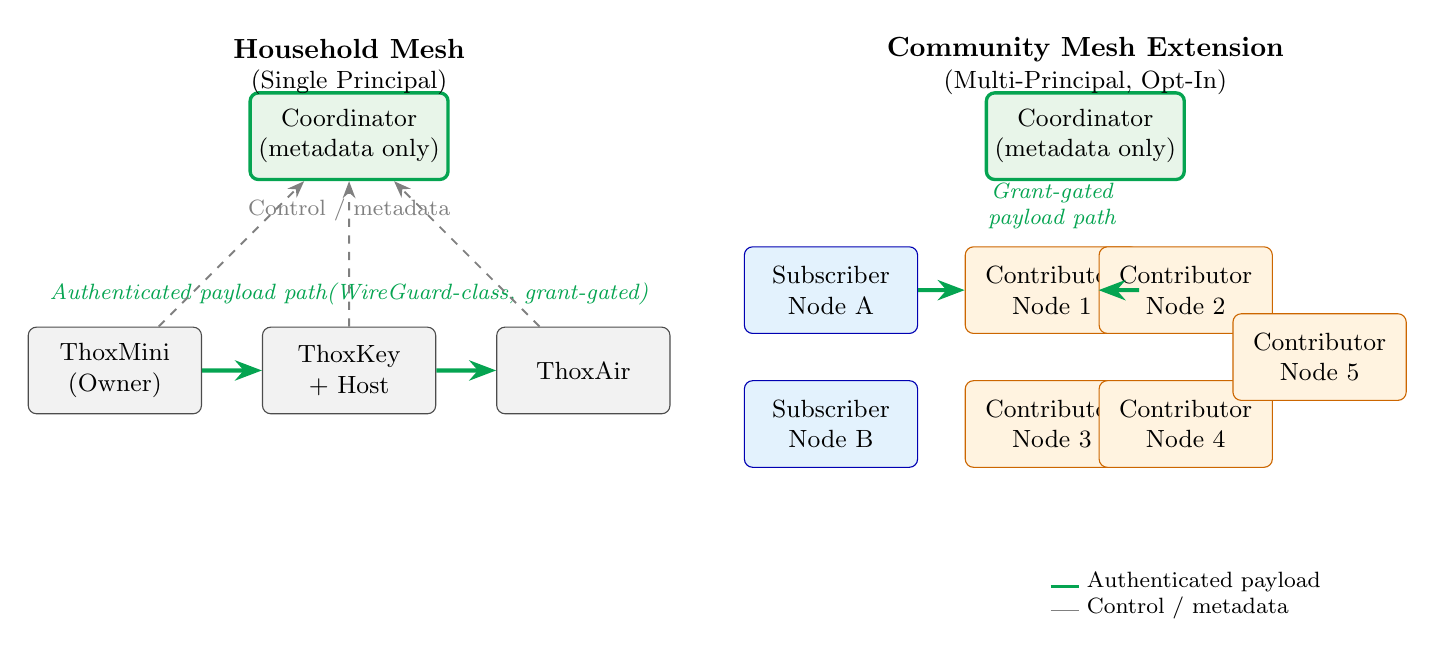
\begin{tikzpicture}[
  node distance=1.2cm and 1.5cm,
  every node/.style={font=\small},
  box/.style={draw, rounded corners=3pt, minimum height=1.1cm, minimum width=2.2cm, align=center, inner sep=3pt},
  coord/.style={box, fill=coordfill, draw=thoxgreen, line width=1.2pt},
  device/.style={box, fill=gray!10, draw=black!70},
  sub/.style={box, fill=subfill, draw=blue!70!black},
  contrib/.style={box, fill=contribfill, draw=orange!80!black},
  payload/.style={->, thoxgreen, line width=1.5pt, >=Stealth},
  control/.style={->, gray, dashed, line width=0.7pt, >=Stealth},
  scale=0.85
]

% ========== Household (left) ==========
\begin{scope}[xshift=0cm]
  \node[coord] (coordH) at (5,8.5) {Coordinator\\(metadata only)};
  \node[device] (d1) at (1.5,5) {ThoxMini\\(Owner)};
  \node[device] (d2) at (5,5) {ThoxKey\\+ Host};
  \node[device] (d3) at (8.5,5) {ThoxAir};
  
  \draw[payload] (d1) -- (d2);
  \draw[payload] (d2) -- (d3);
  \node[above=0.15cm of d2, thoxgreen, font=\footnotesize\itshape] {Authenticated payload path\\(WireGuard-class, grant-gated)};
  
  \draw[control] (d1) -- (coordH);
  \draw[control] (d2) -- (coordH);
  \draw[control] (d3) -- (coordH);
  \node[below=0.1cm of coordH, gray, font=\footnotesize] {Control / metadata};
  
  \node[font=\bfseries] at (5,9.8) {Household Mesh};
  \node[font=\small] at (5,9.3) {(Single Principal)};
\end{scope}

% ========== Community (right) ==========
\begin{scope}[xshift=11cm]
  \node[coord] (coordC) at (5,8.5) {Coordinator\\(metadata only)};
  \node[sub] (s1) at (1.2,6.2) {Subscriber\\Node A};
  \node[sub] (s2) at (1.2,4.2) {Subscriber\\Node B};
  \node[contrib] (c1) at (4.5,6.2) {Contributor\\Node 1};
  \node[contrib] (c2) at (6.5,6.2) {Contributor\\Node 2};
  \node[contrib] (c3) at (4.5,4.2) {Contributor\\Node 3};
  \node[contrib] (c4) at (6.5,4.2) {Contributor\\Node 4};
  \node[contrib] (c5) at (8.5,5.2) {Contributor\\Node 5};
  
  \draw[payload] (s1) -- (c1);
  \draw[payload] (c1) -- (c2);
  \node[above=0.1cm of c1, thoxgreen, font=\footnotesize\itshape, align=center] {Grant-gated\\payload path};
  
  % Legend (simplified)
  \node[below=1.2cm of c4, font=\footnotesize, align=left] {
    \textcolor{thoxgreen}{\rule{1.2em}{0.8pt}} Authenticated payload\\
    \textcolor{gray}{\rule[0.3ex]{1.2em}{0.4pt}} Control / metadata
  };
  
  \node[font=\bfseries] at (5,9.8) {Community Mesh Extension};
  \node[font=\small] at (5,9.3) {(Multi-Principal, Opt-In)};
\end{scope}

\end{tikzpicture}
\caption{Household Mesh (left) versus Community Mesh Extension (right). Solid green arrows indicate authenticated, grant-gated payload paths (WireGuard-class). Dashed arrows are control and metadata only. The coordinator remains outside the payload path in both designs. Subscriber nodes (blue) and contributor nodes (orange) appear only in the multi-principal community extension. Research specification; no production community mesh claimed.}
\label{fig:architecture}
\end{figure}



% Figure 2: Pipeline Sharding
\begin{figure}[htbp]
\centering
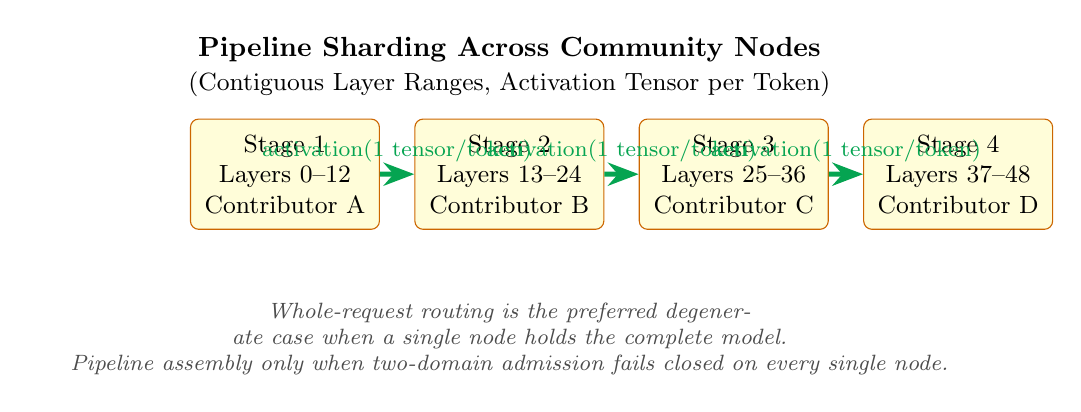
\begin{tikzpicture}[
  stage/.style={draw, rounded corners=3pt, fill=yellow!15, draw=orange!80!black, minimum height=1.4cm, minimum width=2.4cm, align=center, font=\small},
  act/.style={->, thoxgreen, line width=1.8pt, >=Stealth},
  scale=0.95
]
  \node[stage] (s1) at (1.5,2) {Stage 1\\Layers 0--12\\Contributor A};
  \node[stage] (s2) at (4.5,2) {Stage 2\\Layers 13--24\\Contributor B};
  \node[stage] (s3) at (7.5,2) {Stage 3\\Layers 25--36\\Contributor C};
  \node[stage] (s4) at (10.5,2) {Stage 4\\Layers 37--48\\Contributor D};
  
  \draw[act] (s1) -- (s2) node[midway, above, font=\footnotesize, thoxgreen] {activation\\(1 tensor/token)};
  \draw[act] (s2) -- (s3) node[midway, above, font=\footnotesize, thoxgreen] {activation\\(1 tensor/token)};
  \draw[act] (s3) -- (s4) node[midway, above, font=\footnotesize, thoxgreen] {activation\\(1 tensor/token)};
  
  \node[below=0.8cm of s2, font=\footnotesize\itshape, text width=12cm, align=center, color=black!70] 
    {Whole-request routing is the preferred degenerate case when a single node holds the complete model.\\
     Pipeline assembly only when two-domain admission fails closed on every single node.};
     
  \node[above=0.6cm of s2, font=\bfseries] {Pipeline Sharding Across Community Nodes};
  \node[above=0.15cm of s2, font=\small] {(Contiguous Layer Ranges, Activation Tensor per Token)};
\end{tikzpicture}
\caption{Pipeline sharding places contiguous layer ranges on contributor stages. One activation tensor per token crosses each boundary. Whole-request routing remains the preferred degenerate case when a single node holds the complete model. Pipeline assembly occurs only when two-domain admission fails closed on every single node. CALCULATED placement geometry from household admission rules.}
\label{fig:pipeline}
\end{figure}



% Figure 3: Grant DAG
\begin{figure}[htbp]
\centering
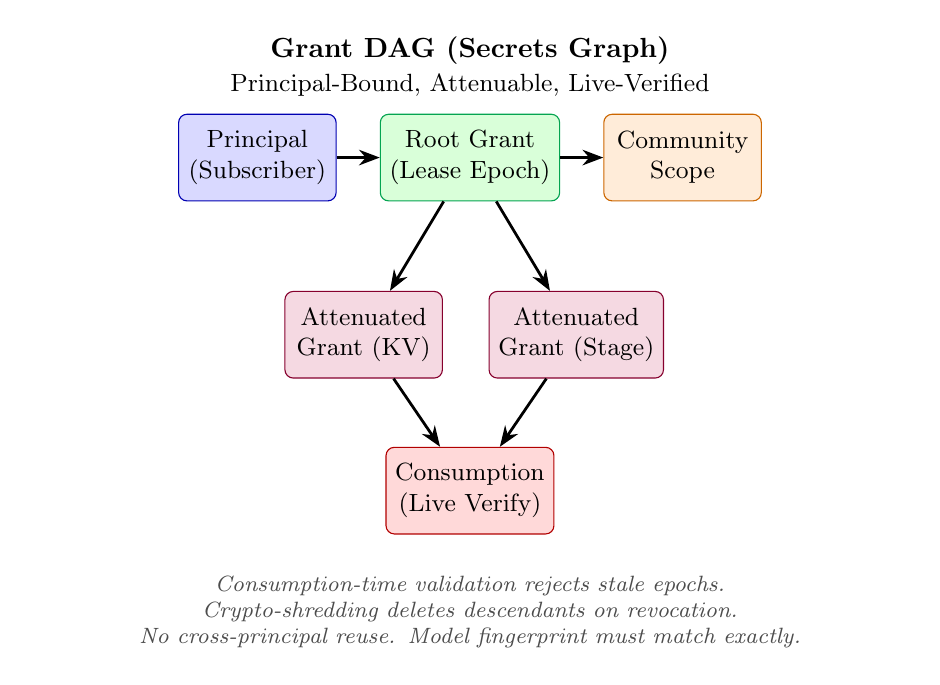
\begin{tikzpicture}[
  node distance=1.4cm,
  grant/.style={draw, rounded corners=3pt, minimum height=1.1cm, minimum width=2.0cm, align=center, font=\small},
  princ/.style={grant, fill=blue!15, draw=blue!70!black},
  root/.style={grant, fill=green!15, draw=thoxgreen},
  scope/.style={grant, fill=orange!15, draw=orange!80!black},
  atten/.style={grant, fill=purple!15, draw=purple!70!black},
  cons/.style={grant, fill=red!15, draw=red!70!black},
  arr/.style={->, >=Stealth, line width=1pt},
  scale=0.9
]
  \node[princ] (p) at (2,6.5) {Principal\\(Subscriber)};
  \node[root] (r) at (5,6.5) {Root Grant\\(Lease Epoch)};
  \node[scope] (sc) at (8,6.5) {Community\\Scope};
  \node[atten] (a1) at (3.5,4) {Attenuated\\Grant (KV)};
  \node[atten] (a2) at (6.5,4) {Attenuated\\Grant (Stage)};
  \node[cons] (c) at (5,1.8) {Consumption\\(Live Verify)};
  
  \draw[arr] (p) -- (r);
  \draw[arr] (r) -- (sc);
  \draw[arr] (r) -- (a1);
  \draw[arr] (r) -- (a2);
  \draw[arr] (a1) -- (c);
  \draw[arr] (a2) -- (c);
  
  \node[below=0.4cm of c, font=\footnotesize\itshape, text width=11cm, align=center, color=black!70]
    {Consumption-time validation rejects stale epochs. Crypto-shredding deletes descendants on revocation.\\
     No cross-principal reuse. Model fingerprint must match exactly.};
     
  \node[above=0.5cm of r, font=\bfseries] {Grant DAG (Secrets Graph)};
  \node[above=0.1cm of r, font=\small] {Principal-Bound, Attenuable, Live-Verified};
\end{tikzpicture}
\caption{Grant DAG (Secrets Graph): principal-bound, attenuable grants with consumption-time validation and crypto-shredding on revocation. No cross-principal reuse. Model fingerprint must match exactly. Consumption rejects stale lease epochs.}
\label{fig:grantdag}
\end{figure}


\end{document}
